\section{Dead Ends}

Some approaches we had to give up, as they did not work out well or went in the wrong direction. Still, a short summary of what we did shall be given here.

\subsection{SARIMA model for global CO\textsubscript{2} levels}

We put a lot of effort in predicting global \co levels, until we noticed that this would not help us directly. We thought that we could see a drop in \co levels but this is actually not the case. Even with the emissions going down, levels still rise. The forecast itself is still pretty good we think, it perfectly follows the seasonality of actual \co levels. Our work was not for nothing though, as we could apply our knowledge on SARIMA models later to forecast indicators.

%\begin{figure}[h!]
%	\centering
%	\subfloat[Raw driving data]{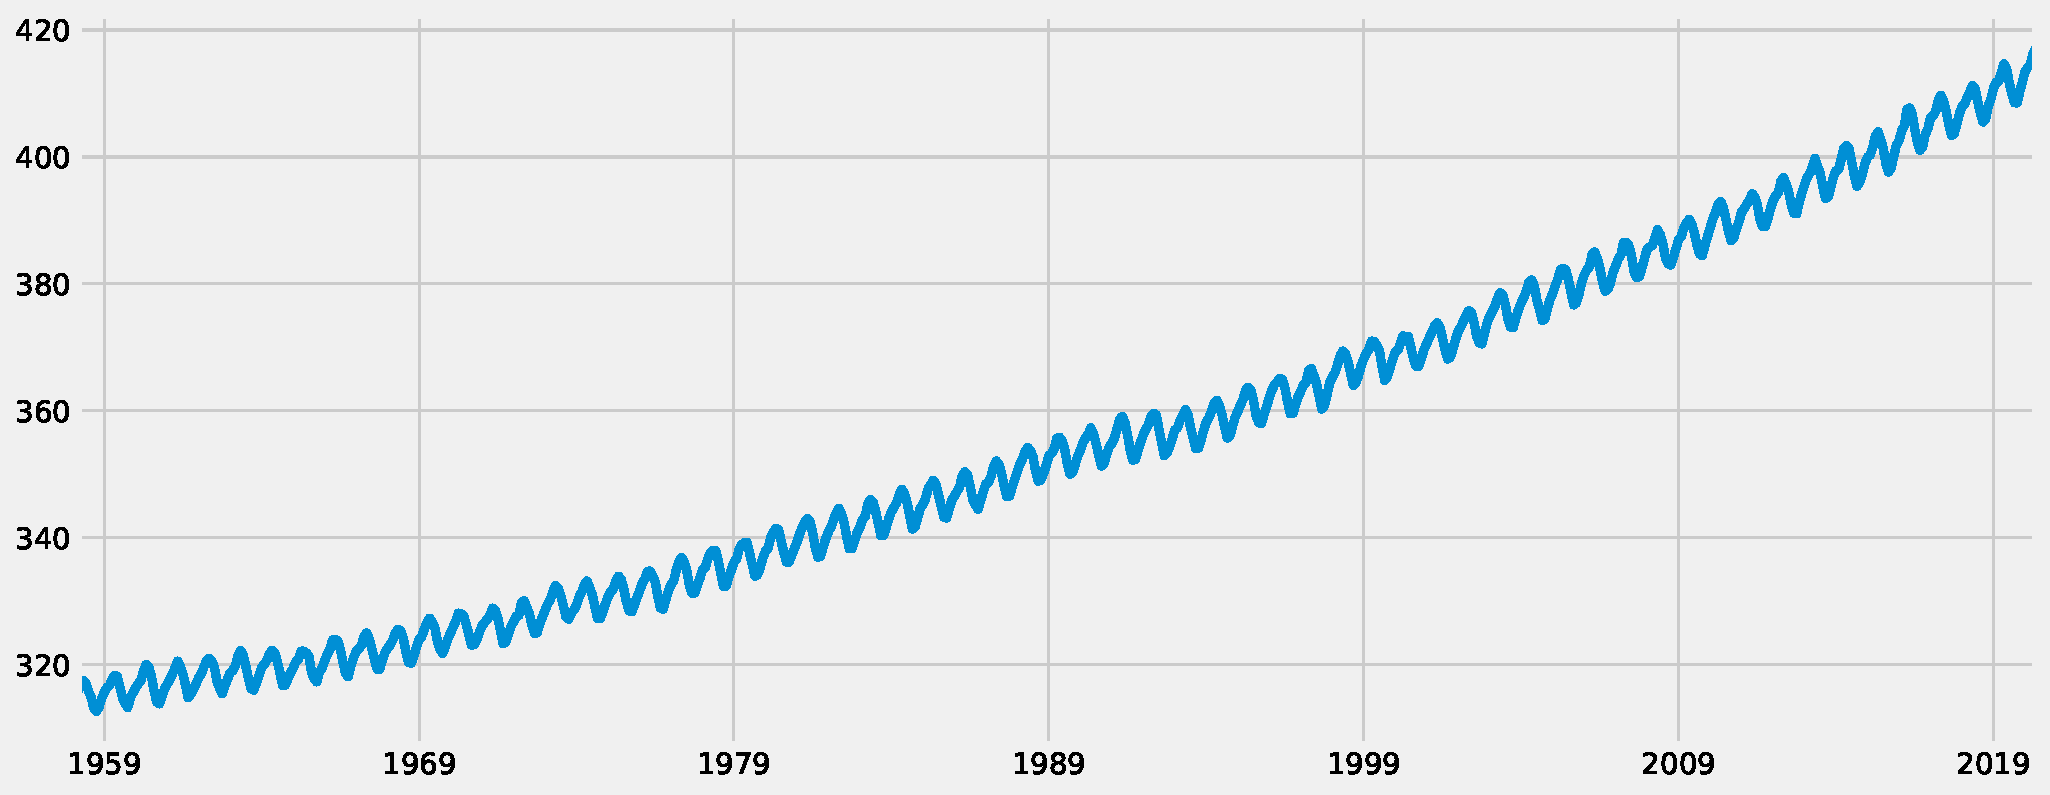
\includegraphics[width=0.4\linewidth]{../sarima_co2/allCO2data.pdf}}
%	\hspace{1cm}
%	\subfloat[Driving data with moving average]{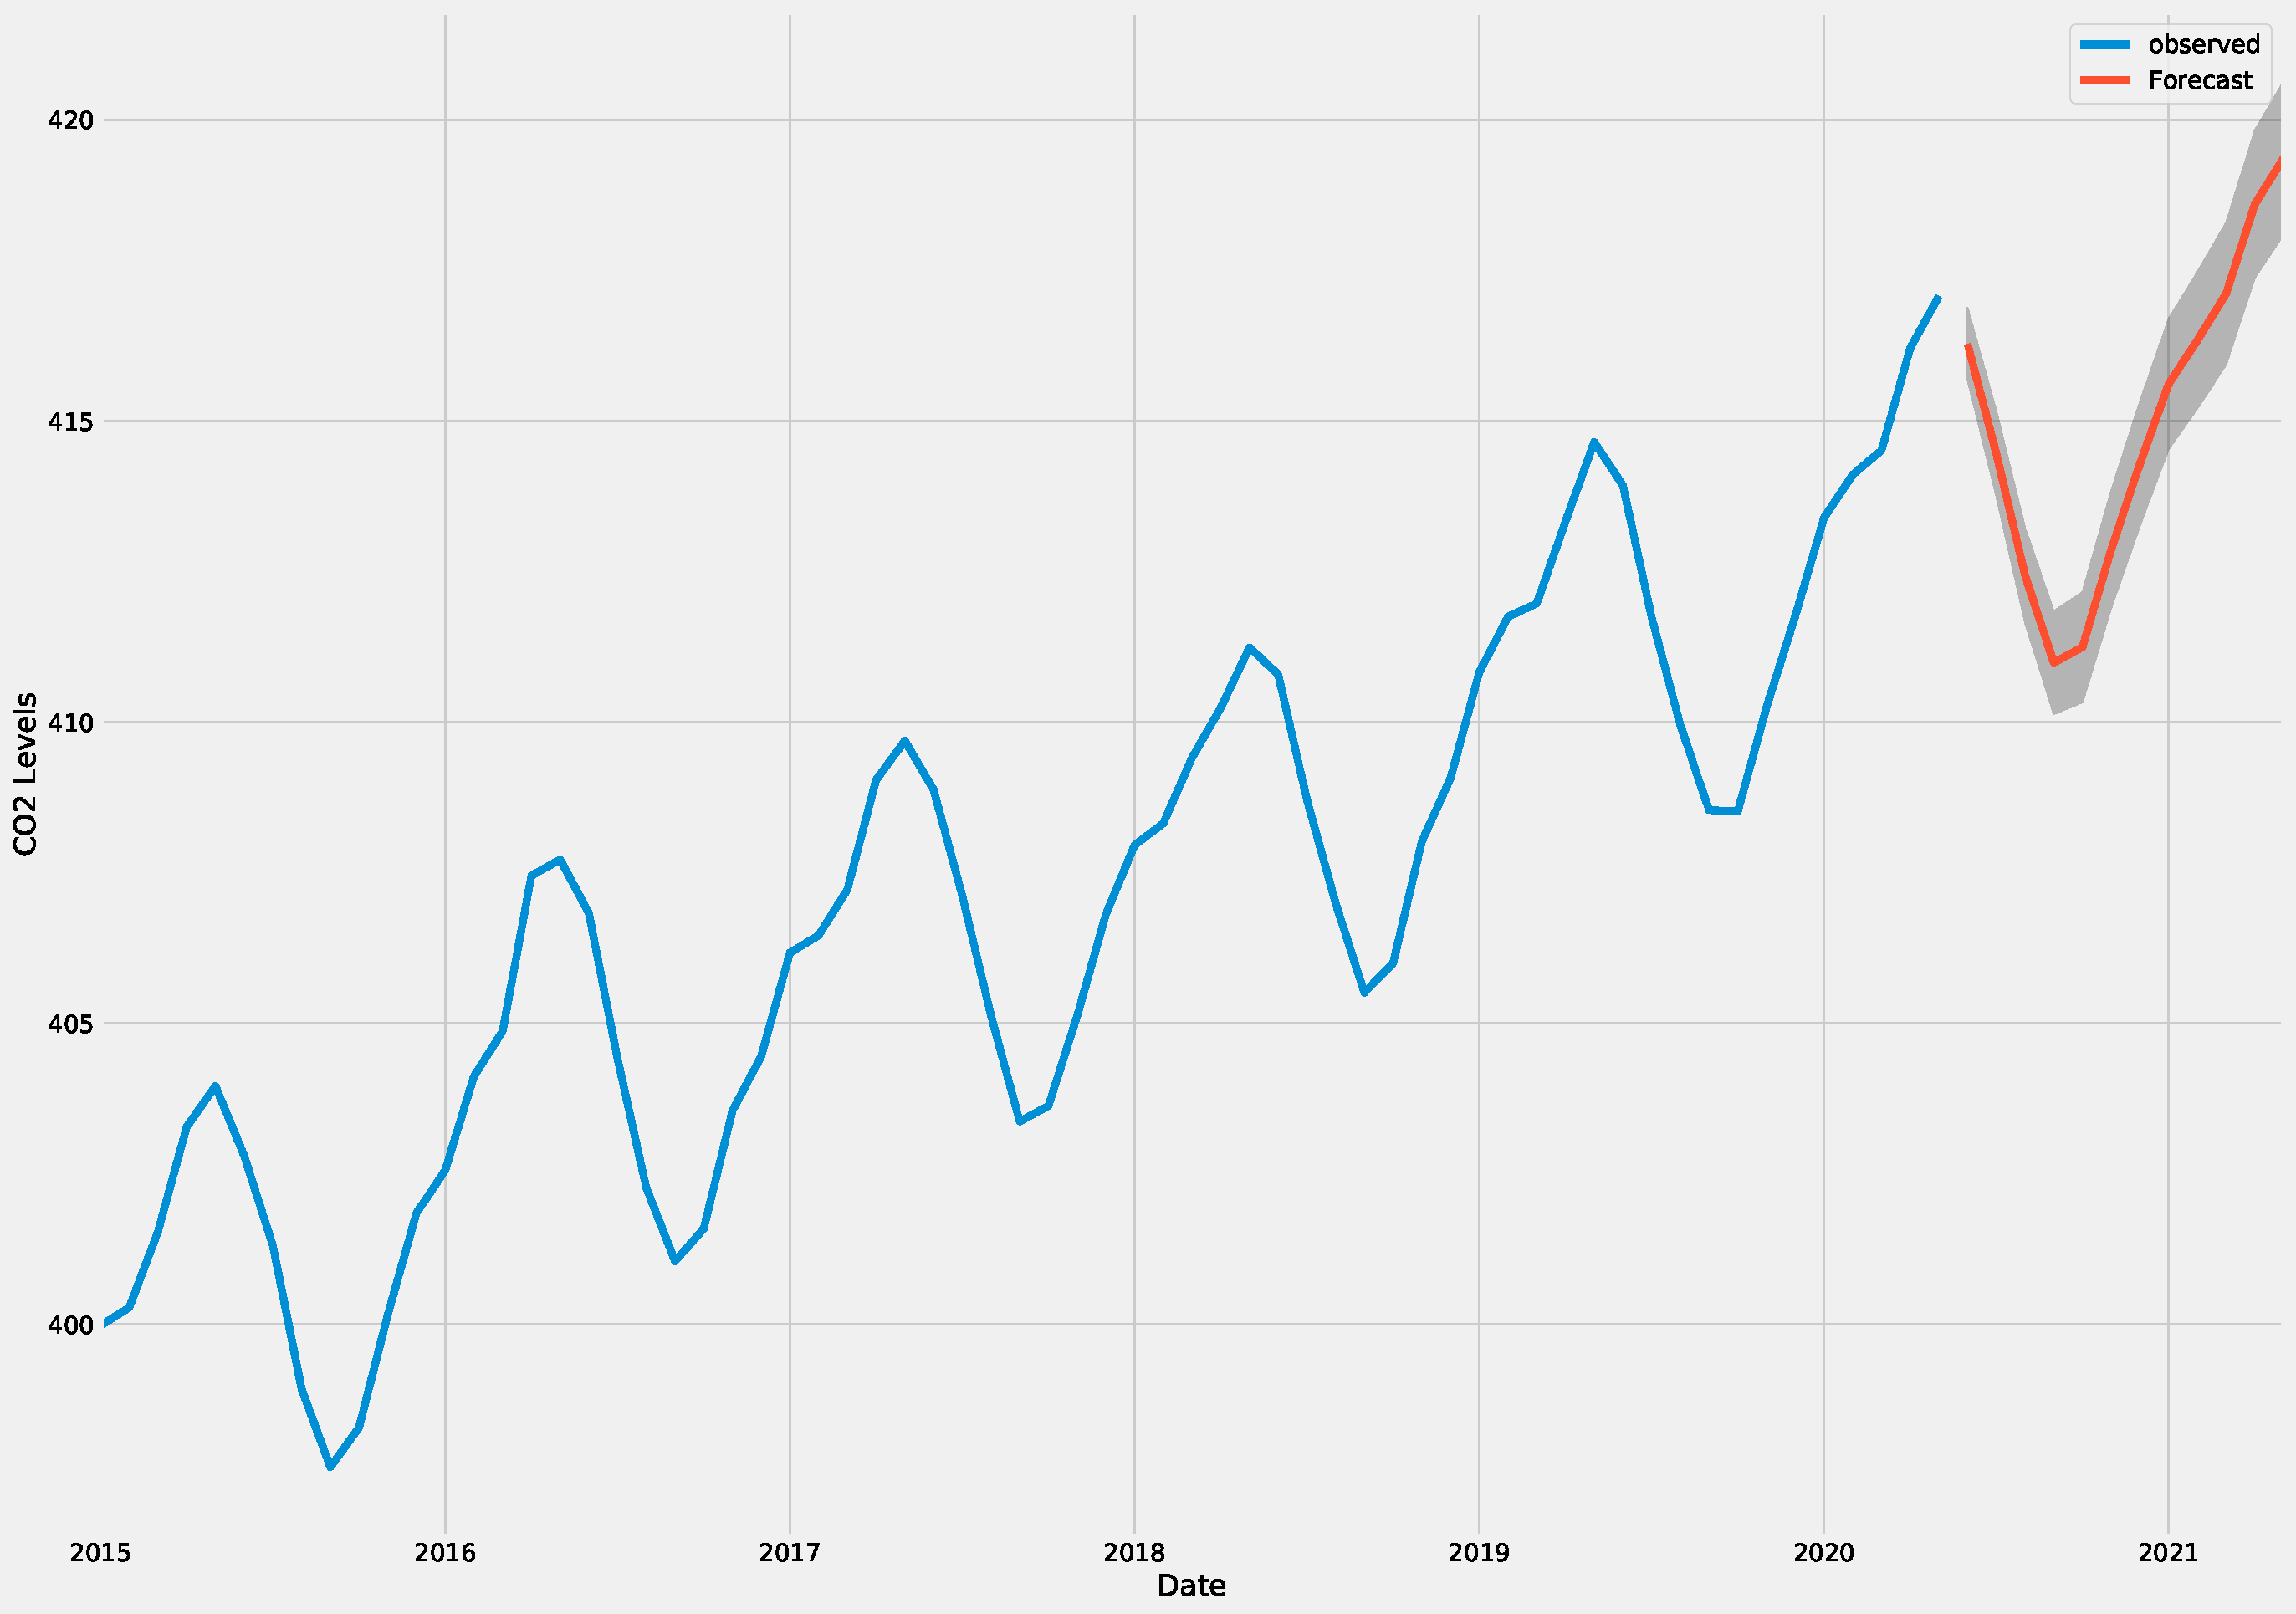
\includegraphics[width=0.4\linewidth]{../sarima_co2/dyn_pred_forecast.pdf}}
%	\caption{Mobility data. A steep drop is visible for all countries.}
%	\label{fig:driving}
%\end{figure}

\begin{figure}[hb!]
	\centering
	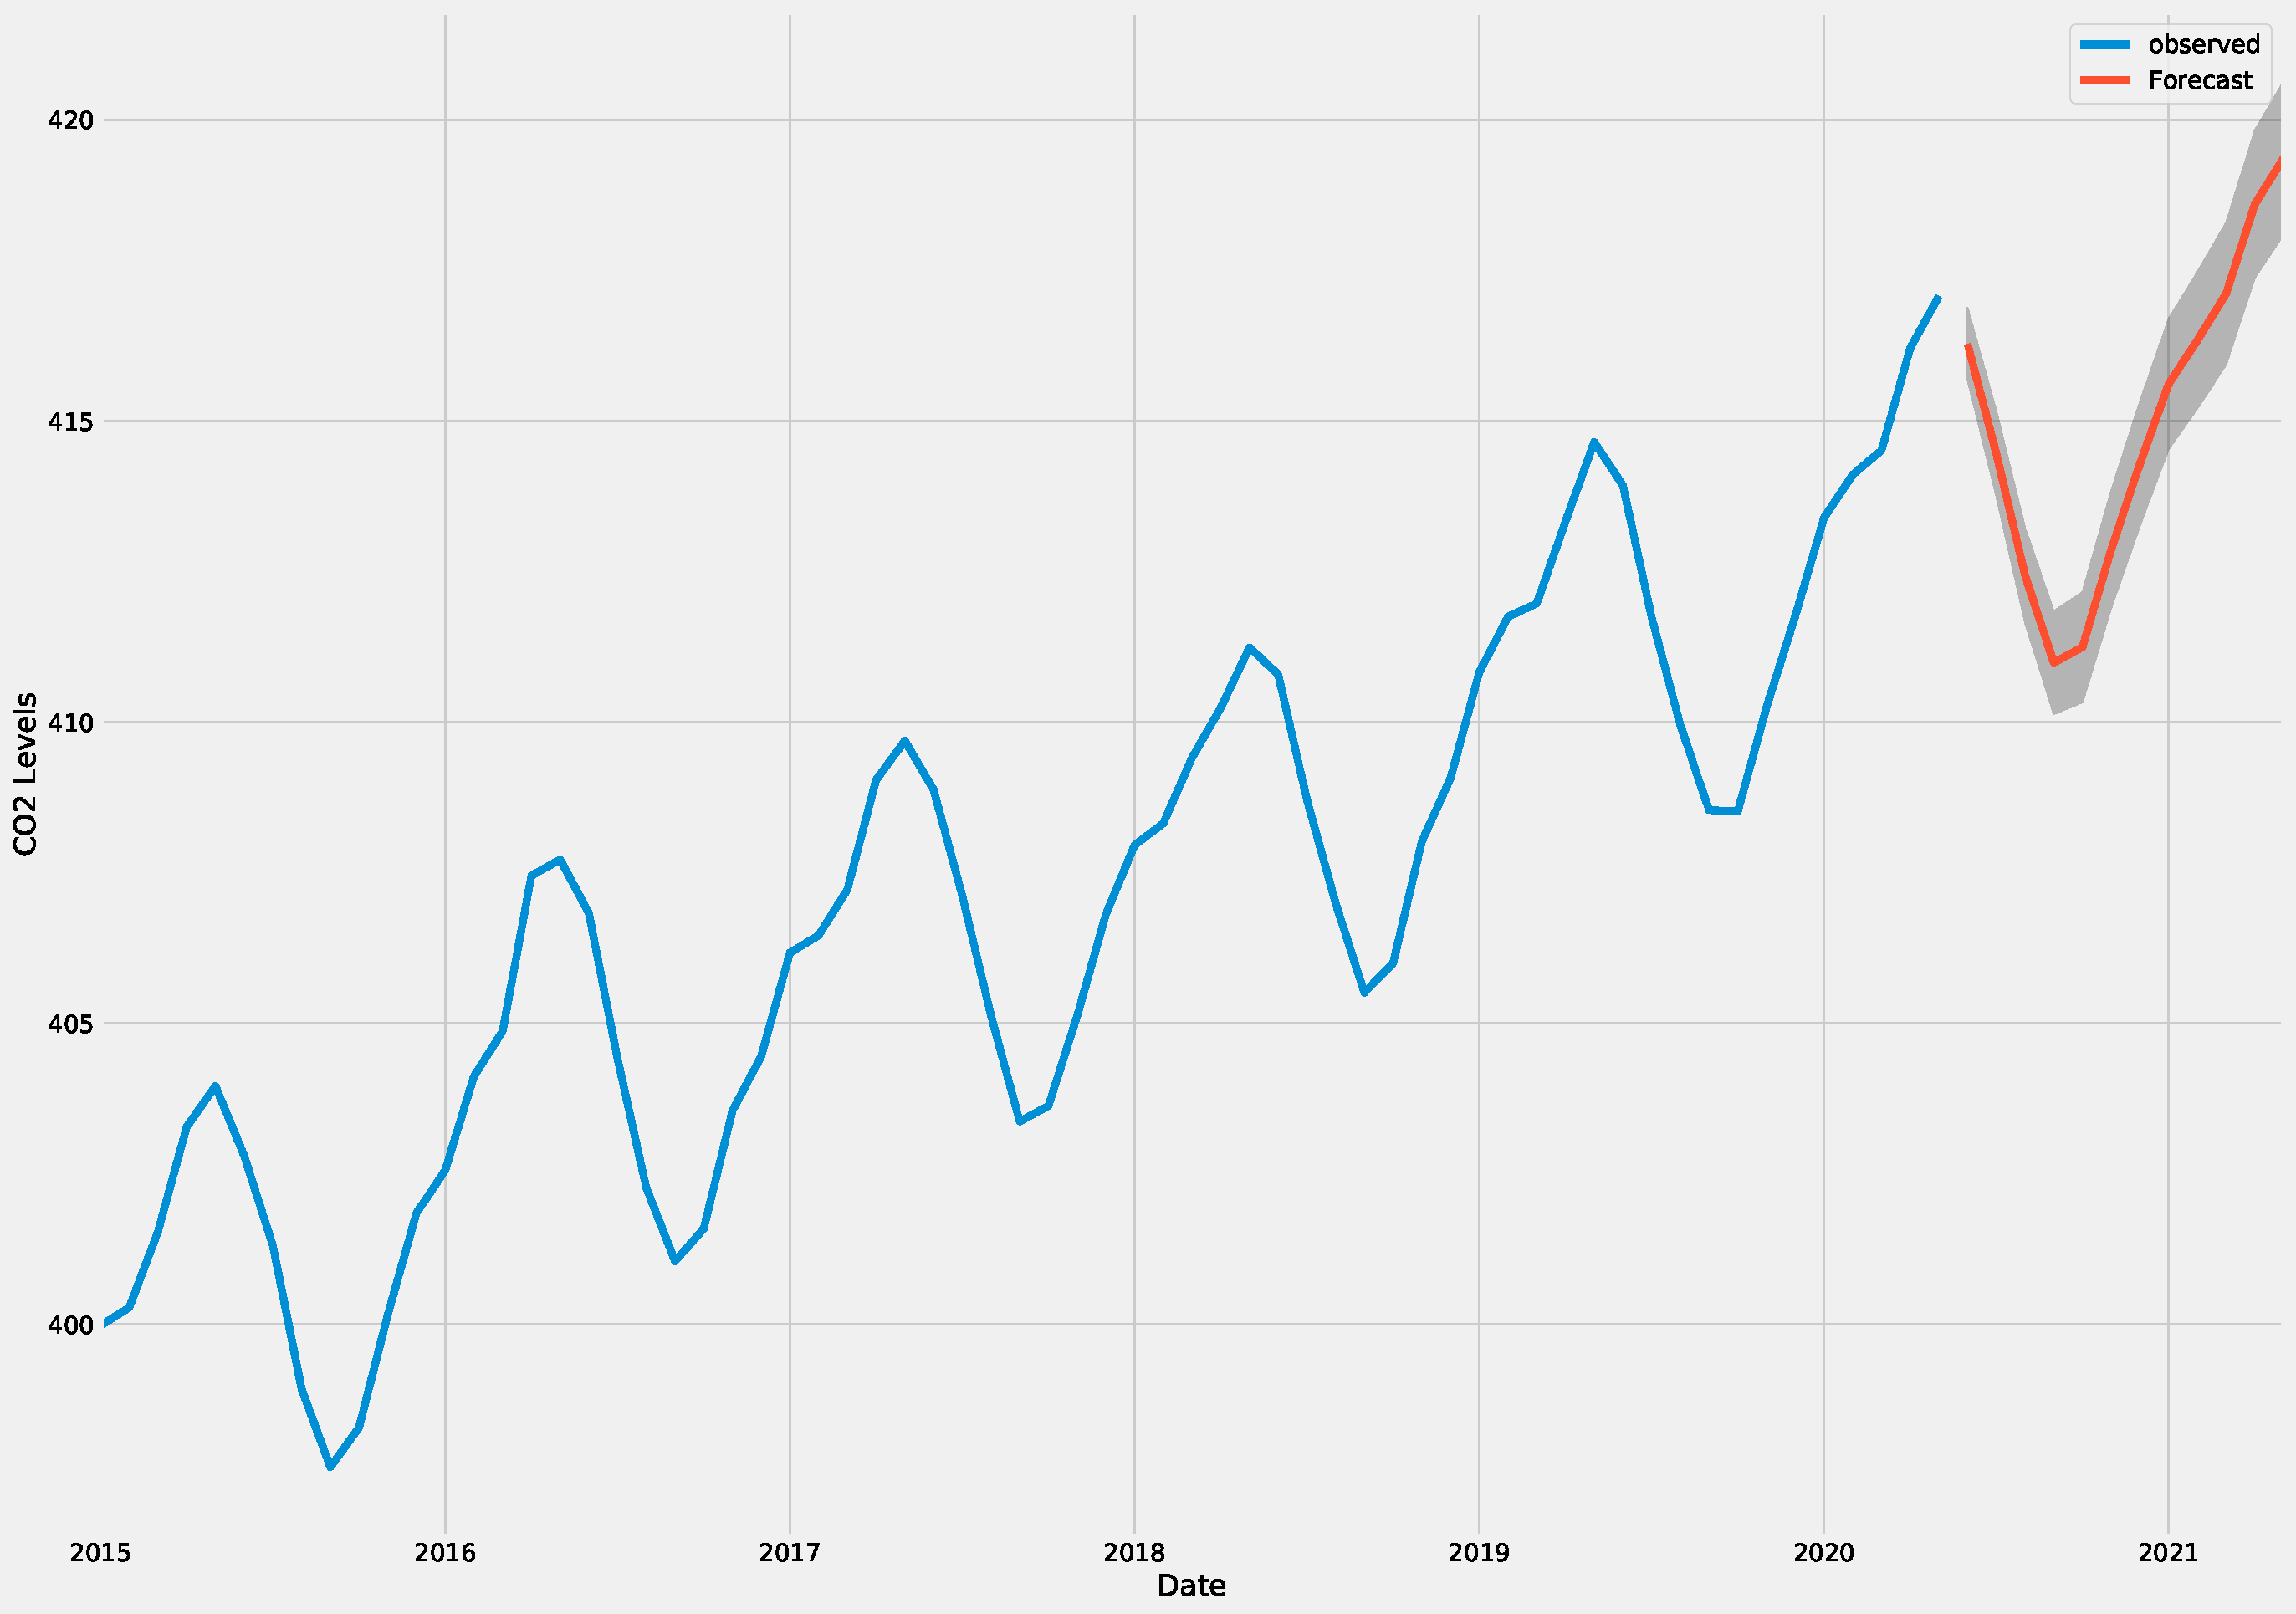
\includegraphics[width=0.7\linewidth]{../sarima_co2/dyn_pred_forecast.pdf}
	\caption{\co levels from 2015 until beginning of 2020 in blue and a forecast to mid 2021 in orange, including an area of uncertainty in gray.}
	\label{fig:flights}
\end{figure}

\subsection{Weather data}

We also tried to gather satellite precipitation data for the whole world and even had correspondence to data scientists at NASA to explain to us how to access the data. However, when we turned away from our first approach by going with \co levels, we also did not need weather data anymore. Precipitation mainly affects \co levels, not \co emissions. Therefore, this also became a dead end.

\subsection{Recursive Neural Network for predicting athmospheric \co concentration in the future}

One of our first attempts was to predict atmospheric \co emissions in the future by use of pure time series \co concentration data.  Since a mostly generic RNN architecture would serve as a basic structure for other time series predictions as well, we implemented a RNN that could be used for several problems. Only predicting one outcome per cycle and recursively using this result for predicting multiple time steps was not successful at all, even after some optimization steps. An example for one of those results can be seen in the following Figure \ref{fig:RNN1}. In this particular case, a RNN with a single hidden layer with 500 neurons and ten steps as inputs was used.

\begin{figure}[hb!]
	\centering
	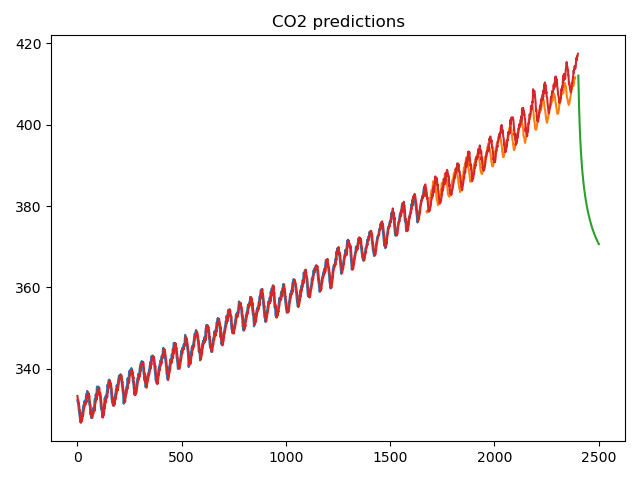
\includegraphics[width=0.7\linewidth]{./RNN_athmospheric _CO2_prediction/500neurons_10_inputs_1_output.jpg}
	\caption{\co First attempt: predicting a single output recursively.}
	\label{fig:RNN1}
\end{figure}

Alternatively, predicting multiple time steps in one single cycle was much more successful. Still, the results which are shown in Figure \ref{fig:RNN2} were not convincing at all. In this case, 1000 neurons within the single hidden layer with five inputs were used. In one step, 100 outputs were predicted.

\begin{figure}[hb!]
	\centering
	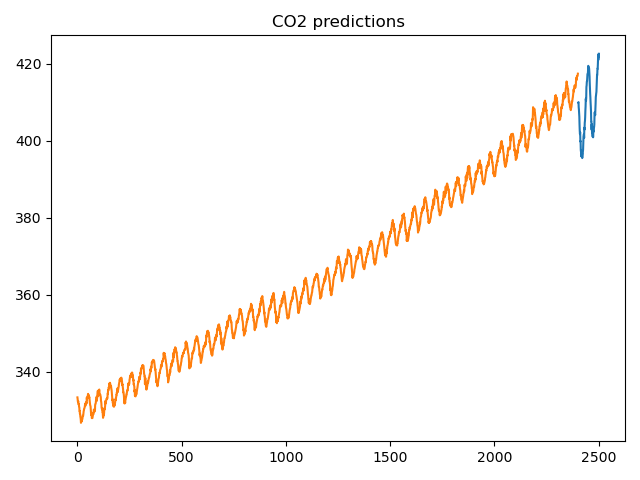
\includegraphics[width=0.7\linewidth]{./RNN_athmospheric _CO2_prediction/1000neurons_5inputs_100_outputs.jpg}
	\caption{\co Predicting multiple steps in the future.}
	\label{fig:RNN2}
\end{figure}

After taking into account knowlegde we gained from the lecture, the reading assignments and discussing the occured issues, we decided to split the time series data into a trend and a seasonal component. The implemented RNN served for predicting the seasonal behavior in the future. This much more convincing result can be seen in Figure \ref{fig:RNN3}. For predicting the trend component, a simple multi layer perceptron was used.

\begin{figure}[hb!]
	\centering
	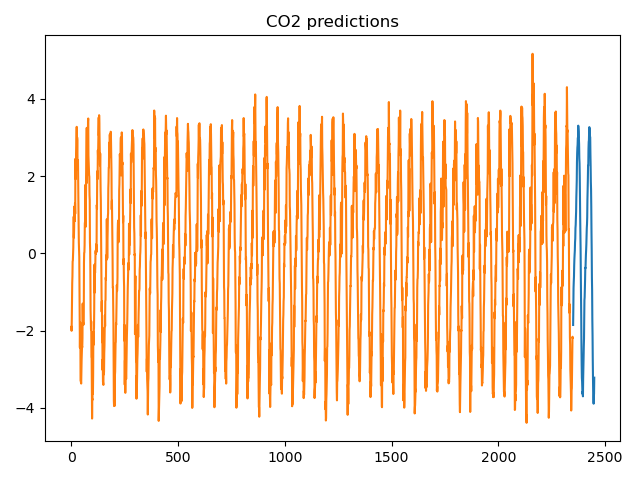
\includegraphics[width=0.7\linewidth]{./RNN_athmospheric _CO2_prediction/seasonal_predictions}
	\caption{\co Predicting only seasonal behavior.}
	\label{fig:RNN3}
\end{figure}
